\documentclass{beamer}

\usepackage[utf8]{inputenc}
\usepackage[T1]{fontenc}
\usepackage[francais]{babel}
\usepackage{graphicx}
\usepackage{multimedia}
\usepackage{url}

\addtobeamertemplate{navigation symbols}{}{
    \usebeamerfont{footline}
    \usebeamercolor[fg]{footline}
    \hspace{1em}
    \insertframenumber/\inserttotalframenumber
}

\usetheme{Warsaw}

	\title{Hand Kinect}
  \author{Elliot Vanegue, Gaëtan Deflandre et Alexis Robache}
  \institute{\large Suivi par :\\ 
  Hazem Wannous et Jean-Philippe Vandeborre}
  \date{\oldstylenums{Novembre 2015}}

\begin{document}
  
  \frame{\titlepage}
  
   \begin{frame}
   	\frametitle{Présentation contexte}
   	Objectif :\\
   	\begin{itemize}
		  \item Détection de la main
		  \item Reconnaissance de la posture de la main
		  \item Modélisation de la main
		  \item Animation de la main
	  \end{itemize}
	  \ \\		
	  \ \\
  	Equipe : 3D-Sam\\
 	\end{frame}
 	
 	\begin{frame}
 	  \frametitle{Présentation contexte}  
 	  Données fourni par la Kinect :
 	  \begin{itemize}
 	    \item Image YUV
 	    \item Image de profondeur
 	  \end{itemize}
 	  \begin{figure}
 	    \begin{center}
 	      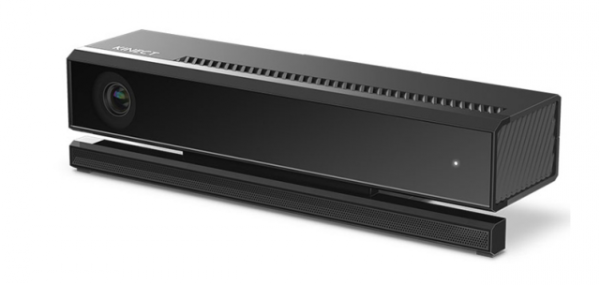
\includegraphics[width=5cm]{images/kinectv2.png}
 	      \vspace{2cm}
 	      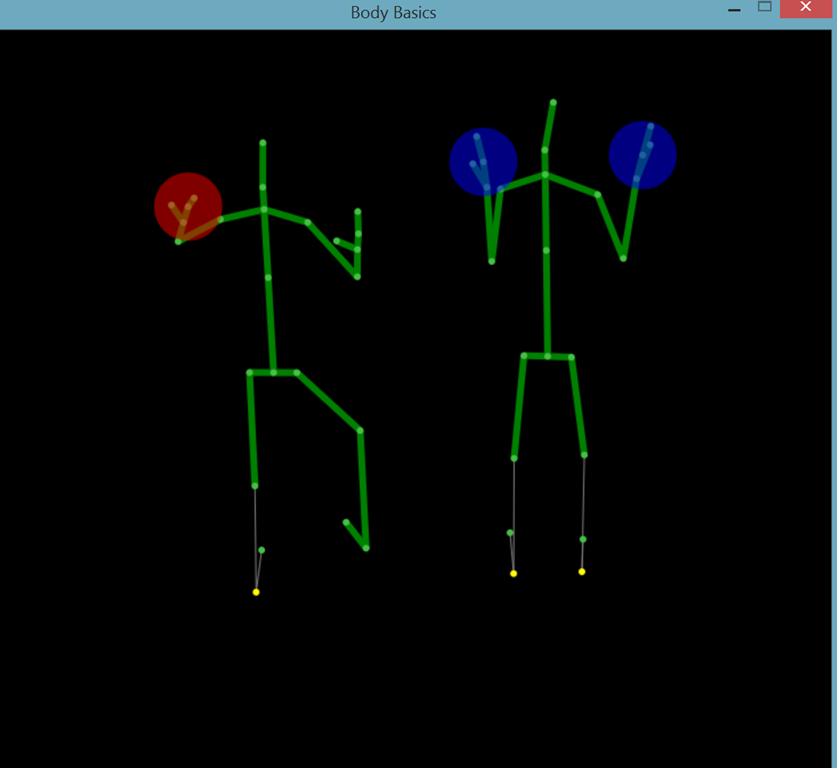
\includegraphics[width=5cm]{images/joints.png}
 	      \label{fig:kinect}
 	    \end{center}
 	  \end{figure}
 	\end{frame}
 	
 	\begin{frame}
 	  \frametitle{Présentation des solutions}
 	  \framesubtitle{Différents types de données}
 	  \begin{figure}
 	    \begin{center}
 	      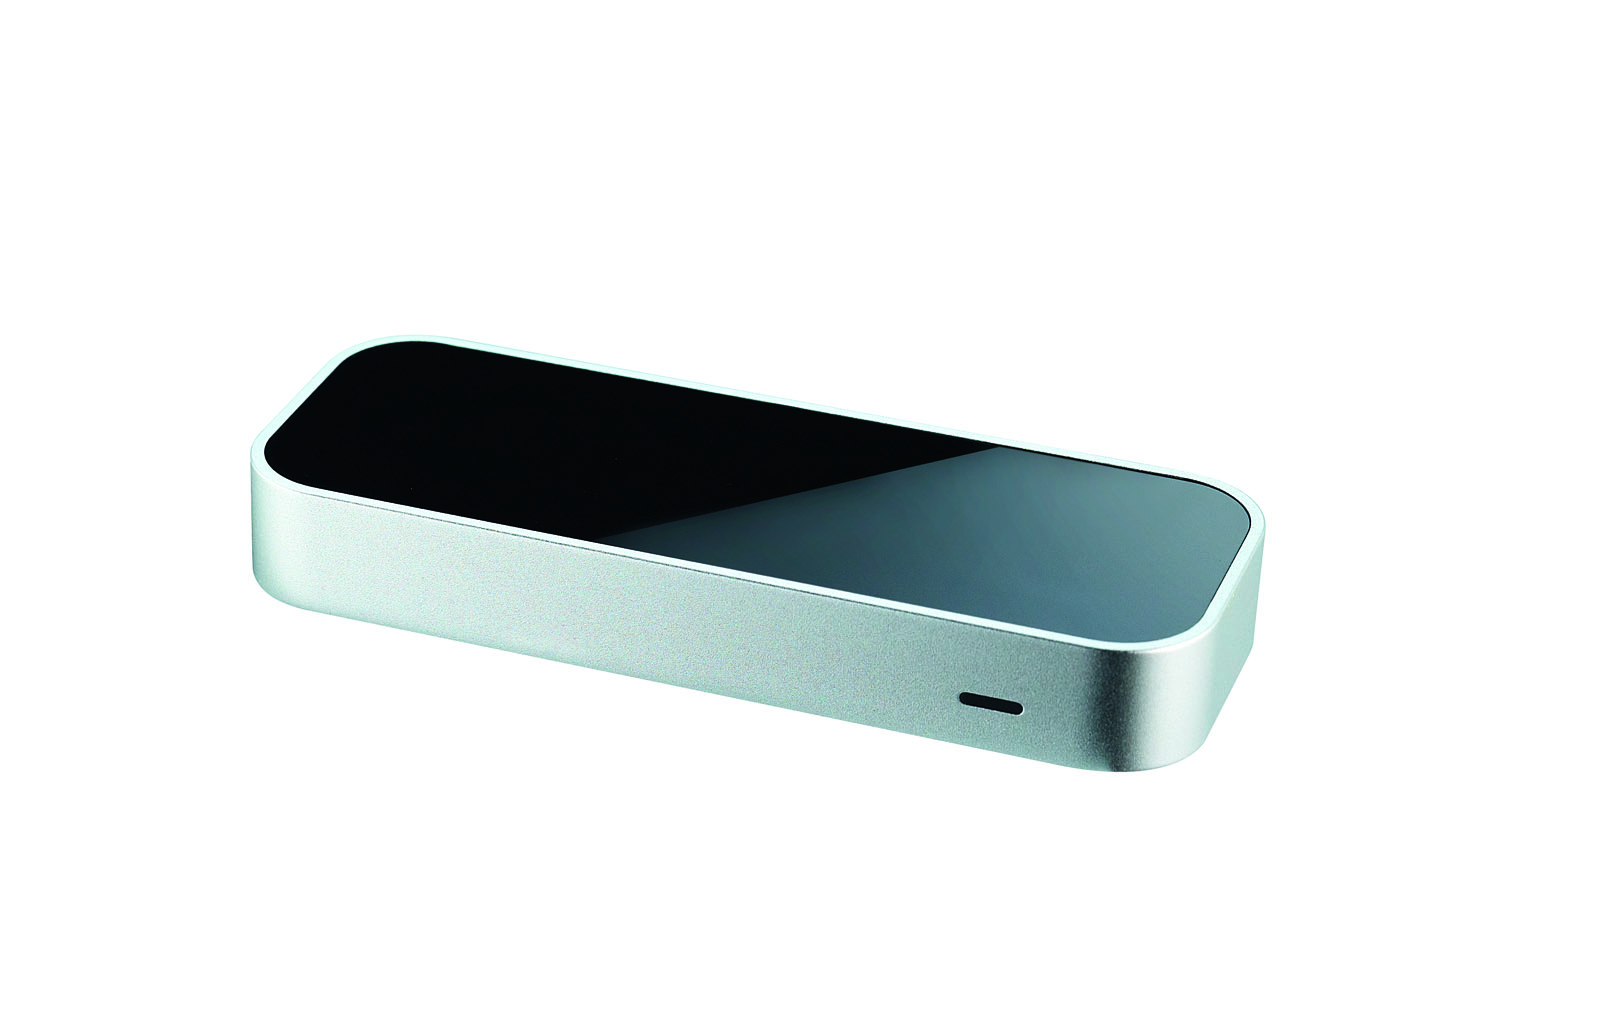
\includegraphics[width=5cm]{images/leapMotion.jpeg}
 	      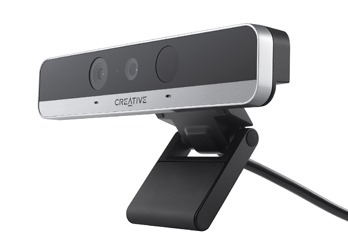
\includegraphics[width=5cm]{images/realsense.jpeg}
 	      \caption{Leap Motion et Realsense}
 	      \label{fig:camera}
 	    \end{center}
 	  \end{figure}
 	\end{frame}
 	
 	\begin{frame}
 	  \frametitle{Présentations des solutions}
 	  \framesubtitle{Détection de la main à partir d'une image couleur}
 	  Algorithme de Viola et Jones
 	  \begin{figure}
 	    \begin{center}
 	      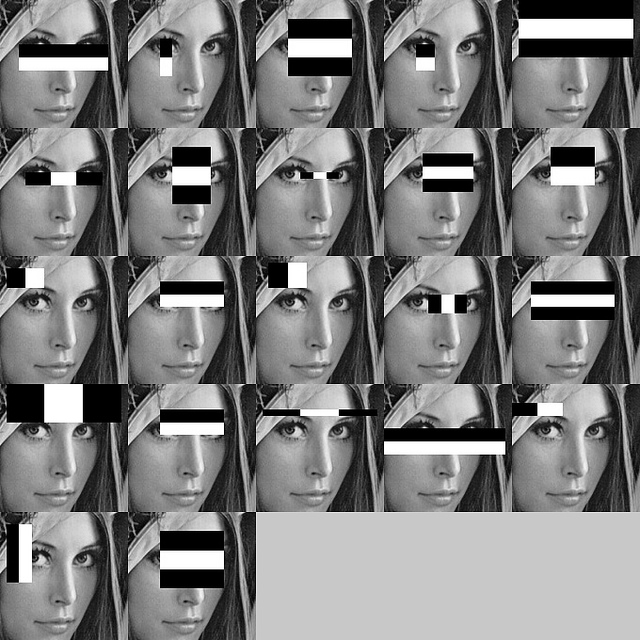
\includegraphics[width=5cm]{images/pseudoHaar.jpg}
 	      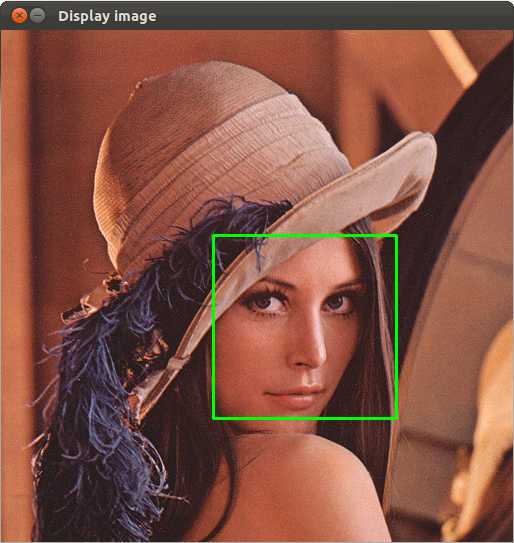
\includegraphics[width=5cm]{images/facedet.png}
 	      \label{fig:pseudoHaar}
 	    \end{center}
 	  \end{figure}
 	  \cite{viola2001jones}
 	\end{frame}
 	
 	\begin{frame}
 	  \frametitle{Présentations des solutions}
 	  \framesubtitle{Détection de la main à partir d'une image couleur}
 	  Détection des doigts de la main
 	  \begin{figure}
 	    \begin{center}
 	      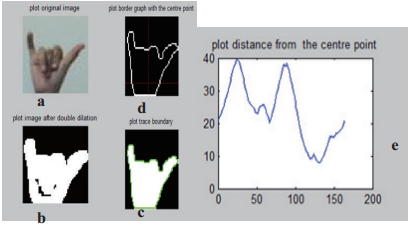
\includegraphics[width=8cm]{images/handHisto.png}
 	      \label{fig:doigts}
 	    \end{center}
 	  \end{figure}
 	\end{frame}
 	
 	\begin{frame}
 	  \frametitle{Présentations des solutions}
 	  \framesubtitle{Détection de la main à partir d'une image de profondeur}
 	  Réutilisation de la méthode utilisé par la Kinect
 	  \begin{figure}
 	    \begin{center}
 	      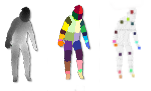
\includegraphics[width=8cm]{images/bodyrecognition.png}
 	      \label{fig:bodyPartRecognition}
 	    \end{center}
 	  \end{figure}
 	  \cite{export:238453}
 	\end{frame}
 	
 	\begin{frame}
 	  \frametitle{Présentations des solutions}
 	  \framesubtitle{Modélisation de la main}
 	  \begin{figure}
 	    \begin{center}
 	      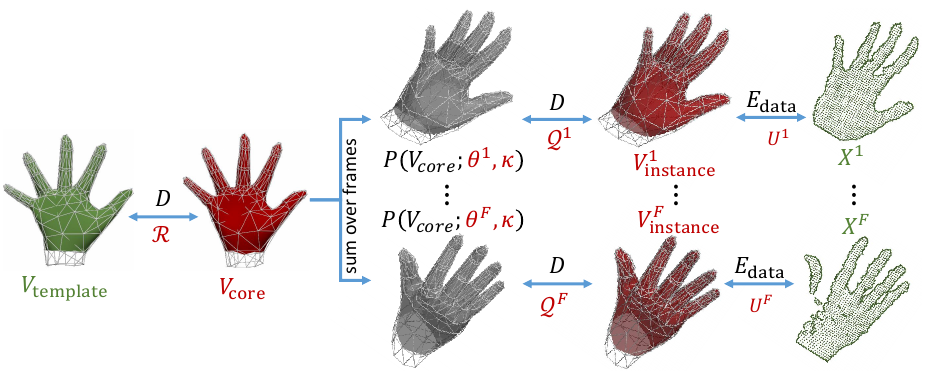
\includegraphics[width=10cm]{images/MethodeModelisation.png}
 	      \label{fig:modelisation}
 	    \end{center}
 	  \end{figure}
 	  \cite{export:217428}
 	\end{frame}
 	
 	\begin{frame}
 	  \frametitle{Prévisionnel du projet}
 	  \begin{figure}[H]
 	    %\begin{center}
 	    \hspace{-10mm}
 	      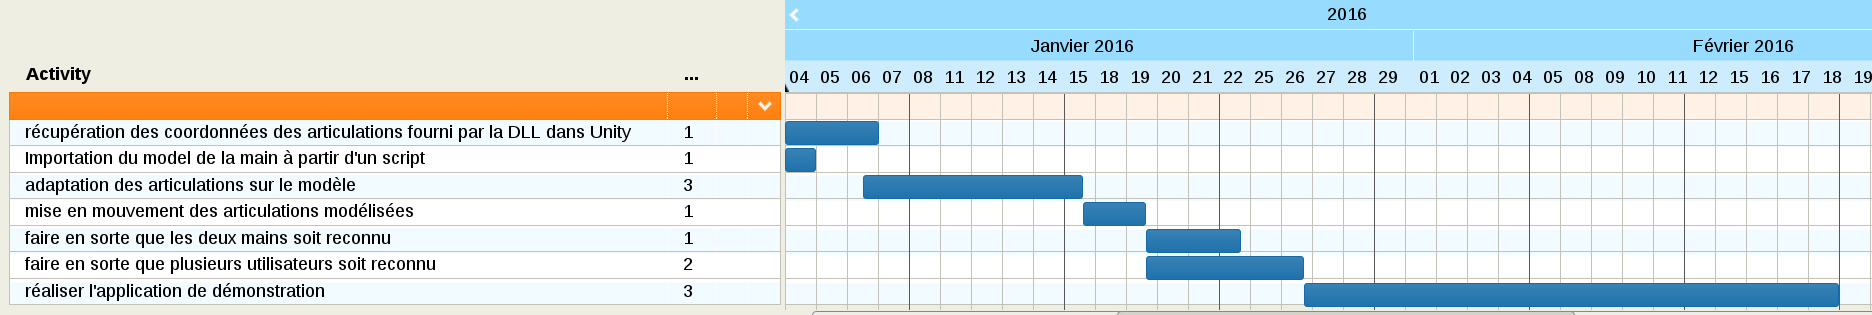
\includegraphics[width=115mm, height=30mm]{images/planning.png}
 	      \label{fig:planning}
 	    %\end{center}
 	  \end{figure}
 	\end{frame}
 	
 	\begin{frame}
 	  \frametitle{Conclusions}
 	  Application de démontration\\
 	  %\url{videos/leapMotion.mp4}
 	  \movie[width=10cm, height=7cm]{Exemple}{videos/leapMotion.mp4}
 	\end{frame}
 	
 	\begin{frame}
 	  \frametitle{Référence}
 	  \bibliographystyle{ieeetr} % or try abbrvnat or unsrtnat or plainnat
    \bibliography{biblio}
 	\end{frame}
 	
\end{document}
